\documentclass[stu,donotrepeattitle]{apa7}
\usepackage[style=apa,sortcites=true,backend=biber]{biblatex}
\usepackage{movie15}
\addbibresource{references.bib}
\title{Using Deep Learning to Detect Epileptic Seizures Through EEG Signals}
\nocite{*}
\shorttitle{Epileptic Seizure Detection}
\author{Anish Goyal}
\authorsaffiliations{{Governor's Honors Program 60}}
\course{Engineering: Computer Programming}
\professor{Anupam Goli}
\duedate{July 1, 2023}
\newcommand{\HRule}{\rule{\linewidth}{0.25mm}}
\setlength\parindent{36pt}
\begin{document}
\maketitle
\newpage

\section{Introduction}
\begin{itemize}
    \item Epileptic seizures are episodes of abnormal electrical activity in the brain that can cause a variety of symptoms, including convulsions, loss of consciousness, and sensory disturbances.
    \item Approximately 1 \% of the world's population suffers from epileptic seizures.   
    \item Seizure prediction is the ability to identify changes in brain activity that may precede a seizure.
    \item This information can be used to prevent seizures by taking medication or adjusting other treatment plans.
    \item Machine learning and deep learning approaches have been used to develop seizure prediction algorithms.
    \item These algorithms can extract features from electroencephalography (EEG) signals that are predictive of seizures.
    \item Some of the most commonly used machine learning and deep learning algorithms for seizure prediction include:
    \begin{itemize}
    \item Support vector machines (SVMs)
    \item Decision trees
    \item Random forests
    \item Artificial neural networks (ANNs)
    \item Convolutional neural networks (CNNs)
    \end{itemize}
    \item Seizure prediction algorithms have been shown to be effective in a variety of clinical settings.
    \item However, there are still challenges that need to be addressed, such as:
    \begin{itemize}
    \item The need for large datasets of EEG signals
    \item The development of more accurate and robust algorithms
    \item The integration of seizure prediction algorithms into clinical practice
    \end{itemize}
\end{itemize}

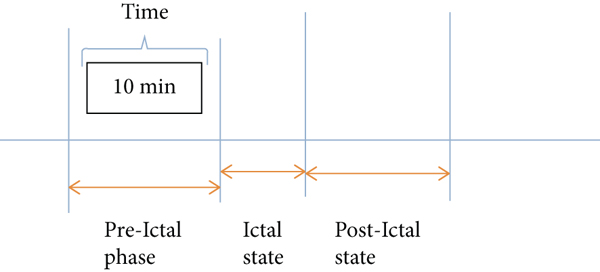
\includegraphics{img/3.jpg}

\section{Types of Networks}

\begin{itemize}

    \item \textbf{Convolutional neural networks (CNNs)} are a type of deep learning algorithm that are well-suited for processing image data. CNNs work by applying a series of convolution operations to the input data, which helps to extract features from the data. These features can then be used to classify the data into different categories.
    
    \item In the article \textit{A Deep Convolutional Neural Network Method to Detect Seizures and Characteristic Frequencies Using Epileptic Electroencephalogram (EEG) Data}, the authors used a CNN to classify EEG signals into two categories: seizure and non-seizure. The CNN was trained on a dataset of EEG signals from patients with epilepsy. The CNN was able to achieve an accuracy of 99.21\% in classifying seizure and non-seizure EEG signals.
    
    \item The authors also used the CNN to identify characteristic frequencies in the EEG signals that were predictive of seizures. They found that the CNN was able to identify frequencies in the range of 4--8 Hz, which are known to be associated with seizures.
    
    \item \textbf{Support vector machines (SVMs)} are another type of machine learning algorithm that can be used for seizure prediction. SVMs work by finding a hyperplane that separates the seizure and non-seizure EEG signals.
    
    \item \textbf{Decision trees} are a simple but effective machine learning algorithm that can be used for seizure prediction. Decision trees work by splitting the data into smaller and smaller groups until each group contains only seizure or non-seizure EEG signals.
    
    \item \textbf{Random forests} are an ensemble learning algorithm that combines multiple decision trees to improve accuracy. Random forests are often used for seizure prediction because they are able to handle noisy data and are relatively easy to interpret.
    
\end{itemize}

\includemovie{4cm}{4cm}{img/2.gif}

\section{Methodology}

\begin{itemize}

    \item Scientists use deep learning to predict epileptic seizures by first collecting EEG data from patients with epilepsy.
    \item The EEG data is then used to train a deep learning model.
    \item The deep learning model learns to identify patterns in the EEG data that are predictive of seizures.
    \item Once the deep learning model is trained, it can be used to predict seizures in real time.
    \item The deep learning model can be used to alert patients with epilepsy before a seizure occurs, giving them time to take preventive measures.
    \item The deep learning model can also be used to improve the accuracy of seizure detection algorithms.
    
    \end{itemize}
    
    Here is a more detailed explanation of each step:
    
    1. \textbf{Collecting EEG data:} EEG data is collected from patients with epilepsy using electrodes that are placed on the scalp. The EEG data records the electrical activity of the brain.
    2. \textbf{Training a deep learning model:} The EEG data is used to train a deep learning model. Deep learning models are a type of machine learning model that can learn complex patterns from data. The deep learning model learns to identify patterns in the EEG data that are predictive of seizures.
    3. \textbf{Predicting seizures in real time:} Once the deep learning model is trained, it can be used to predict seizures in real time. The deep learning model analyzes the EEG data in real time and alerts patients with epilepsy if it detects a pattern that is predictive of a seizure.
    4. \textbf{Alerting patients before a seizure occurs:} The deep learning model can alert patients with epilepsy before a seizure occurs, giving them time to take preventive measures. For example, patients can take medication to prevent the seizure from happening, or they can find a safe place to lie down.
    5. \textbf{Improving the accuracy of seizure detection algorithms:} The deep learning model can also be used to improve the accuracy of seizure detection algorithms. Seizure detection algorithms are used to identify seizures in EEG data. The deep learning model can be used to train seizure detection algorithms to be more accurate.
    
    Scientists are still working on developing deep learning models that can accurately predict epileptic seizures. However, the research in this area is promising, and deep learning models have the potential to revolutionize the way that epileptic seizures are treated.    

\includemovie{4cm}{4cm}{img/1.gif}

\section{Public Datasets Available For Seizure Prediction}

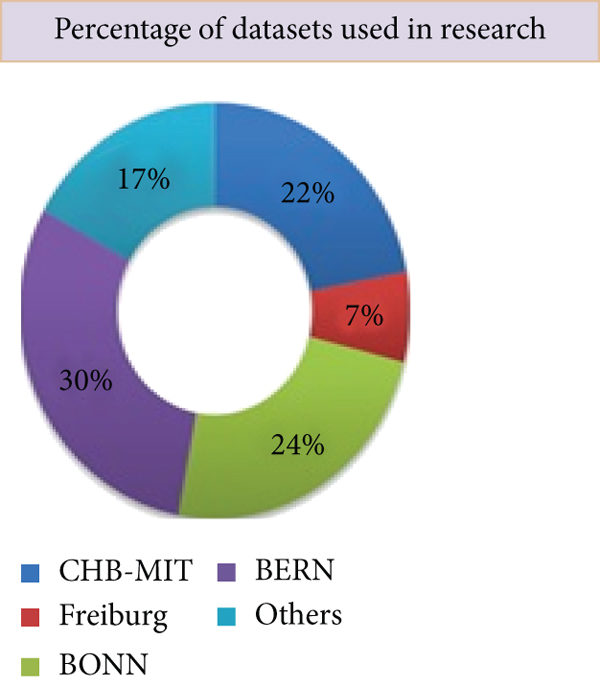
\includegraphics{img/4.jpg}

\printbibliography{}
\end{document}